\documentclass[../Main.tex]{subfiles}


\begin{document}


\chapter{LES SÉRIES DE FONCTIONS}
\intro{
\textbf{Prérequis}
\begin{itemize}
\item Les séries numériques 
\item L'étude fonctions réelles
\end{itemize} 
\textbf{Objectifs}
\begin{itemize}
\item Savoir étudier une fonction définit par une série numérique définit par un paramètre 
\end{itemize}
}{
Dans ce chapitre, On considère une suite des fonctions $(f_n)_{n\in\NN}$ définit sur une ensemble $A \subset \CC$ et à valeurs réelles. On étudiera dans ce chapitre la fonction $f$ définit par : $ f : x \rightarrow \sum_{n=0}^\infty f_n(x) $ sous le contraint de convergence. On verra les outils qui vont nous aider à étudier cette fonction : 
\begin{itemize}
	\item Leur limites/continuité : pour avoir une idée sur les branches infinies 
	\item Leurs Dérivés/variations : qui nous indiquent la variation / la convexité…
\end{itemize}
}

\section{Les quatre modes de convergences }

\subsection{Convergence Simple  }
\defn{Convergence Simple}{
	Lorsque pour tout réel x dans $A$ la série numérique : $\sum f_n(x)$ converge vers un réel noté $f(x)$, on dit que la série des fonctions : $\sum f_n$ converge simplement vers la fonction : $f : x \rightarrow f(x)$ et on écrit : 
	\[ \sum f_n  \xrightarrow{CVS} f \]
}

\exm{}{
Montrez que la série des fonctions de terme générale : $(\frac{x}{n(1+2nx)})_{n\in\NN^*} $ est simplement convergente sur $\RR^+$ : 
\sol
Soit $x\geq 0$ : 
\\ Étudions la convergence de série $\sum_n \frac{x}{n(1+2nx)}$ , On a : \[  \frac{x}{n(1+2nx)} \sim \frac{1}{n^2} \]
Ainsi la série : $ \sum_n \frac{1}{n^2} $ converge (série classique de Riemann - voir corr \eqref{cor:Serie-Ref} ), alors la série $\sum_n \frac{x}{n(1+2nx)}$ est également convergente. En conclut la convergence simple de série.
}

\subsection{Convergence Absolue }
\defn{Convergence Absolue}{
	Lorsque pour tout réel x dans $A$ la série numérique : $\sum |f_n(x)|$ converge vers un réel, on dit que la série des fonctions : $\sum f_n$ converge Absolument. Et si c'est le cas, alors la série converge aussi simplement sur $A$ vers une fonction : $f : x \rightarrow f(x)$ et on écrit : 
	\[ \sum f_n  \xrightarrow{CVA} f \]
}

\exm{}{
Montrez que la série des fonctions de terme générale : $(\frac{x}{n(1+2nx^2)})_{n\in\NN^*} $ est Absolument convergente sur $\RR$ : 
\sol
Soit $x\in\RR$ : 
\\ Étudions la convergence de série $\sum_n \frac{x}{n(1+2nx^2)}$ , On a : \[  \left| \frac{x}{n(1+2nx^2)} \right| \sim \frac{1}{|x|\times n^2} \]
Ainsi la série : $ \sum_n \frac{1}{n^2} $ converge (série classique de Riemann - voir corr \eqref{cor:Serie-Ref} ), alors la série $\sum_n \frac{x}{n(1+2nx^2)}$ est également convergente. En conclut la convergence absolue de série.
}

\subsection{Convergence Normale  }
\defn{Convergence Normale }{
	Lorsque la série numérique : $\sum ||f_n||^A_{\infty}$ converge vers un réel, on dit que la série des fonctions : $\sum f_n$ converge Normalement. Et si c'est le cas, alors la série converge aussi simplement sur $A$ vers une fonction : $f : x \rightarrow f(x)$ et on écrit : 
	\[ \sum f_n  \xrightarrow{CVN} f \]
}

\meth{Étude directe}{
	Il suffit de calculer la norme infinie en fonction de $n$, par les méthodes enseignées en terminale (table de variation), puis on examine la convergence de la série : $\sum ||f_n||^A_{\infty}$ : cela nous donne une condition nécessaire et suffisante de convergence normale.
}

\exm{}{
soit la série des fonctions de terme générale : $(\frac{x}{n(1+2nx)})_{n\in\NN^*} $, Étudier la convergence normale de cette série sur $\RR^+$.
\sol
Posons pour tout $n\in \NN^*$ la fonction $ u_n : x \rightarrow \frac{x}{n(1+2nx)} $. soit $n\in \NN^*$ ,la fonction $u_n$ est dérivable sur $\RR^+$ ainsi sa dérivée est : $ u'_n(x) = \frac{1}{n(1+2nx)^2} $, donc la fonction est croissante, ainsi sa borne-sup est $\displaystyle ||u_n||^{\RR^+}_{\infty}=\lim_{x\rightarrow +\infty} u_n(x)=\frac{1}{2n^2}$
}

\meth{En utilisant des conditions suffisantes}{
Dans les exercices, on rencontre souvent des questions type : (Mq la série converge normalement / Mq la série ne converge pas normalement). C'est pour cela qu'on préfère d'utiliser les conditions suffisantes parce qu'ils sont faciles à montrer : 
\begin{itemize}
	\item S'il existe une suite $(\alpha_n)_{n\in\NN}$  tq : 
	\begin{enumerate}
		\item $\forall x \in A \tq |f_n(x)| \leq \alpha_n$
		\item la série : $\sum_n \alpha_n $ converge 
	\end{enumerate}
	Alors la série des fonctions $\sum_n f_n$ converge normalement

	\item S'il existe une suite $(\alpha_n)_{n\in\NN}$  tq : 
	\begin{enumerate}
		\item $\forall x \in A \tq |f_n(x)| \geq \alpha_n$
		\item la série : $\sum_n \alpha_n $ diverge 
	\end{enumerate}
	Alors la série des fonctions $\sum_n f_n$ ne converge pas normalement
\end{itemize}
}

\exm{}{
Mq la série des fonctions $\sum_n e^{-x\sqrt{n}}$ converge normalement sur $[1,+\infty[$.
\sol
on a clairement pour tout réel $x\geq 1 \tq e^{-x\sqrt{n}} \leq e^{-\sqrt{n}} $  
la série $\sum_n e^{-\sqrt{n}} $ est convergente (il suffit de voir que $ e^{-\sqrt{n}} = o(\frac{1}{n^2}) $ et appliqué une règle de comparaison vu en  \eqref{thm:Régles de comparaison (series) }). \\
Cela montre la convergence normale de série.
}

\subsection{Convergence Uniforme  }
\defn{Convergence Uniforme -- Suite de fonctions}{
	soit une suite des fonctions $ (u_n)_{n\in\NN} $ définit sur une ensemble $B\subset\RR$. On dit que la suite converge uniformément vers une fonction $u:x\in A\rightarrow u(x)$ lorsque : 
	\[    \forall \epsilon>0 \ \exists N_{\epsilon}\in \NN \tq \forall n\geq N_{\epsilon} \text{ On a : } \forall x\in A \tq |u_n(x) - u(x)| < \epsilon \] 
}

\defn{Convergence Uniforme -- Série de fonctions}{
	Lorsque la suite des fonctions : $\big( \sum_{k=0}^{n} f_k \big)_{n\geq0}$ converge \textbf{Uniformément} vers une fonction $f$, on dit que la série des fonctions : $\sum f_n$ converge Uniformément. Et si c'est le cas, alors la série converge aussi simplement sur $A$ vers une fonction : $f : x \rightarrow f(x)$ et on écrit : 
	\[ \sum f_n  \xrightarrow{CVU} f \]
}

\meth{Convergence normale}{
La convergence Normale entraîne la convergence Uniforme.
\\ Il suffit alors d'établir la convergence normale (qui nous amène à une série numérique) pour montrer la convergence uniforme.
}
\exm{}{
Dans l'exemple précédent, la série des fonctions $\sum_n e^{-x\sqrt{n}}$ converge normalement sur $[1,+\infty[$ , et alors, elle converge uniformément sur $[1,+\infty[$
}

\meth{Convergence du Reste}{
Pour que la série $\sum_n f_n$ converge uniformément, il faut et il suffit que le reste de série converge uniformément vers la fonction nulle. c.-à-d. :
\[ \sum_n f_n \xrightarrow{CVU} f \textbf{ \ \ \  SSI   \ \ \ : } \big| \big| \sum_{k=n}^{+\infty} f_n  \big| \big|_\infty^A \longrightarrow 0 \] 
}

\exm{}{
L'exemple le plus classique est des séries de fonctions alternées : \\
Soit la série des fonctions $\sum_n \frac{(-1)^n}{n^x}$ ,Mq, elle converge uniformément sur $[\frac{1}{2},+\infty[$ .
\sol 
Soit $x \in [\frac{1}{2},+\infty[$ la série $\sum_n \frac{(-1)^n}{n^x}$  converge étant une série alternée (voir propt \eqref{thm:CSSA}), d'où la convergence simple de série des fonctions. \\
La convergence simple nous permet d'utiliser \textbf{la méthode de convergence de reste} , car le reste existe. \\
On peut majorer le reste $\big(\sum_{k=n+1}^{\infty} \frac{(-1)^k}{k^x}\big)_{n\geq 1}$ en utilisant l'extension de \eqref{thm:CSSA}  on a pour tout réel $x\in [\frac{1}{2},+\infty[$ :
\[ 	\sum_{k=n+1}^{\infty} \frac{(-1)^k}{k^x}	 \leq \frac{1}{(n+1)^x} \leq \frac{1}{(n+1)^{\frac{1}{2}}} \]
Ainsi cela montre que : 
\[ \big|\big|\sum_{k=n+1}^{\infty} \frac{(-1)^k}{k^x} \big|\big|_{\infty}^{[\frac{1}{2},+\infty[} \leq \frac{1}{(n+1)^{\frac{1}{2}}} \longrightarrow 0 \]
D'où la convergence uniforme de série.
}


\section{Étude pratique d'une série des fonctions }
Dans cette section, on conserve toujours les notations de l'Introduction de chapitre. Pour les exemples, on considère la fonction dite \textbf{Zeta de Riemann} définit par : 
\[ \zeta : x \longleftarrow \zeta(x) = \sum_{n=1}^{+\infty} \frac{1}{n^x}\]
\paragraph{Domaine de Définition : } 
On rappelle que d'après corr \eqref{cor:Serie-Ref} - Série Référentielle de Riemann, la série  $\sum_{n} \frac{1}{n^x}$ converge ssi $x>1$. Et donc c'est notre domaine de définition.
Énonçons dans ce qui suit les théorèmes qui permettent l'étude de cette fonction et les appliquons sur elle-même.

\subsection{Limite d'une série des fonctions}

\thm{Théorème de limite}{
soit $a\in\bar{A}$,  Lorsque les conditions suivantes sont vérifiées :
\begin{enumerate}
\item La fonction $f$ est bien définie sur $A$.
\item Les fonctions $f_n$ admettent une limite en $a$ .
\item La série des fonctions $\sum_n f_n$ converge uniformément vers $f$.
\end{enumerate}
On a le résultat suivant : 
\begin{itemize}
\item La série  $\sum_n \lim_{x\rightarrow a} f_n(x)$ converge
\item La fonction $f$ admet une limite en $a$
\item La formule d'inversion : 
\end{itemize}
\begin{equation}\label{eq:INV-LS}
	  \sum_{n=0}^{+\infty} \lim_{x\rightarrow a} f_n(x) = \lim_{x\rightarrow a} \sum_{n=0}^{+\infty}  f_n(x)
\end{equation}
}

\exm{}{
\textbf{Limite en $+\infty$ :} \\
Considérons la partie $A=[2,+\infty[$ : un voisinage de $+\infty$.
\\ On a :
\begin{enumerate}
\item La fonction Zêta est bien définie sur $A$ 
\item Soit $n\in\NN^*$ : la fonction $ x \longrightarrow \frac{1}{n^x}$ admet une limite en $+\infty$ qu'on notera $l_n$ ... un calcul simple nous donne : 
\[ l_n = \fparts{1}{ : n=1}{0}{\text{non}} \]
\item La série converge normalement sur  $[2,+\infty[$ en effet : 
\[ \forall x\in\RR \ \ : \ \ \frac{1}{n^x} \leq \frac{1}{n^2} \text{ \ \ et \ \ } \sum_n \frac{1}{n^2} \text{ une série numérique convergente }  \]
\\ donc la série converge uniformément sur  $[2,+\infty[$
\end{enumerate} 
On conclut alors la formule d'inversion $\lim-\Sigma$ :
	\[ \lim_{x\longrightarrow +\infty }= \sum_{n=1}^{+\infty} l_n = 1 \]
\newline
\textbf{Limite en $1$ :} \\ 
Ici, on n'a pas de convergence uniforme sur un voisinage de $1$, donc on cherche la limite manuellement se dépendre de théorème de limite.
\sol
Soit $A>0$ , on a : $\sum_n \frac{1}{n}$ diverge donc il existe un entier $n\in\NN$ tq :
\[ \sum_{k=1}^n \frac{1}{k} > 2A \]
Ensuite, on sait pour chaque $k\in \{1,..,n\}$ : $\lim_{x\longrightarrow 1}\frac{1}{k^x} = \frac{1}{k}$ \\
Donc il existe $\alpha>0$ tq pour tout $x\in[1,1+\alpha[$ : 
	\[ \frac{1}{k^x} \geq \frac{1}{k} - \frac{A}{n} \]
D'où pour tout $x\in[1,1+\alpha[$ :  
	\[ \zeta(x) \geq \sum_{k=1}^n \frac{1}{k^x} \geq \sum_{k=1}^n \frac{1}{k} - \sum_{k=1}^n \frac{A}{n} \geq 2A - A = A \]
Ce qui montre que $\zeta$ diverge vers $+\infty$ en $x=1$.
}

\subsection{Continuité d'une série des fonctions}

\thm{Théorème de continuité}{
Lorsque les conditions suivantes sont vérifiés :
\begin{enumerate}
\item La fonction $f$ est bien définie sur $A$.
\item Les fonctions $f_n$ sont continues sur $A$.
\item La série des fonctions $\sum_n f_n$ converge uniformément vers $f$.
\end{enumerate}
On a le résultat suivant : 
\begin{itemize}
\item La fonction $f$ est continue sur $A$.
\end{itemize}
}

\exm{}{
Montrons la continuité de la fonction Zêta sur chaque intervalle $[a,+\infty[$ avec $a$ un réel supérieur strictement à $1$.
\sol 
soit $a$ un réel supérieur strictement à $1$ ,On a : 
\begin{enumerate}
\item La fonction $\zeta$ est bien définie sur $[a,+\infty[$ (voir l'introduction de section)
\item soit $n\in\NN^*$, La fonction $x \longrightarrow \frac{1}{n^x}$ étant une composée des fonctions usuelle (exponentielle avec une fonction affine) est continue sur $[a,+\infty[$ 
\item La série converge normalement sur  $[a,+\infty[$ en effet : 
\[ \forall x\in\RR \ \ : \ \ \frac{1}{n^x} \leq \frac{1}{n^a} \text{ \ \ et \ \ } \sum_n \frac{1}{n^a} \text{ une série numérique convergente }  \]
\\ donc la série converge uniformément sur  $[a,+\infty[$
\end{enumerate}
Puis les conditions de théorème sont tous vérifiés, on déduit alors la continuité de Zêta sur  $[a,+\infty[$.
\\ Puisque $\zeta$ est continue sur $[a,+\infty[, \ \forall a>0$ alors elle est continue sur $]0,+\infty[$.(voir sous-section III.5 pour comprendre plus ce genre de raisonnement)
}

\subsection{Dérivés d'une série des fonctions}

\thm{Théorème de Dérivée première}{
Lorsque les conditions suivantes sont vérifiés :
\begin{enumerate}
\item La fonction $f$ est bien défini sur $A$.
\item Les fonctions $f_n$ sont de $C^1$ sur $A$ .
\item La série des fonctions $\sum_n f'_n$ converge uniformément vers $f$.
\end{enumerate}
On a le résultat suivant : 
\begin{itemize}
\item La série  $\sum_n  f_n $ converge uniformément sur $A$
\item La fonction $f$ est de classe $\class^1$ sur $A$
\item La formule d'inversion : 
\end{itemize}
\begin{equation}\label{eq:INV-DS}
\sum_{n=0}^{+\infty}  f'_n = \left( \sum_{n=0}^{+\infty}  f_n \right)' 
\end{equation} 
}

 
\exm{}{
Montrons que la fonction Zêta est de classe $\class^1$ sur chaque intervalle $[a,+\infty[$ avec $a$ un réel supérieur strictement à $1$.
\sol
soit $a$ un réel supérieur strictement à $1$ ,On a : 
\begin{enumerate}
\item La fonction $\zeta$ est bien défini sur $[a,+\infty[$ (voir l'introduction de section)
\item soit $n\in\NN^*$, La fonction $x \longrightarrow \frac{1}{n^x}$ étant une composée des fonctions usuelle (exponentielle avec une fonction affine) est de classe $\class^1$ sur $[a,+\infty[$  et sa dérivée est égale à $ \frac{-\ln(n)}{n^x}$ 
\item La série des dérivées converge normalement sur  $[a,+\infty[$ en effet : 
\[ \forall x\in\RR \  :  \ \left| \frac{-\ln(n)}{n^x} \right| \leq \frac{1}{\ln(n)^{-1}n^a} \text{  \ et \ \ } \sum_n \frac{1}{\ln(n)^{-1}n^a} \text{ une série numérique convergente \eqref{cor:Serie-Ref} }  \]
\\ donc la série des dérivés converge uniformément sur  $[a,+\infty[$
\end{enumerate}
Puis les conditions de théorème sont tous vérifiés, on déduit alors la fonction Zêta est de classe $\class^1$ sur  $[a,+\infty[$.
\\ Puisque $\zeta$ est de classe $\class^1$ sur $[a,+\infty[, \ \forall a>0$ alors, elle est de classe $\class^1$ sur $]0,+\infty[$.(voir sous-section III.5 pour comprendre plus ce genre de raisonnement)
\\ Ainsi l'expression de Sa dérivée est : 
\[\forall x\in \RR^{+}_* \ \ : \ \ \zeta'(x) = \sum_{n=1}^{+\infty} \frac{-\ln(n)}{n^x} \] 
\\ On remarque bien que la dérivée est négative, la fonction Zêta et alors décroissante sur $ \RR^{+}$.
}

\thm{Théorème des Dérivés supérieurs}{
Lorsque les conditions suivantes sont vérifiés :
\begin{enumerate}
\item La fonction $f$ est bien définie sur $A$.
\item Les fonctions $f_n$ sont de classe $\class^{\infty}$ sur $A$ .
\item La série des fonctions $\sum_n f^{(p)}_n$ converge uniformément vers $f$, pour tout entier $p\geq0$.
\end{enumerate}
On a le résultat suivant : 
\begin{itemize}
\item La série  $\sum_n  f_n $ converge uniformément sur $A$
\item La fonction $f$ est de classe $\class^{\infty}$ sur $A$
\item La formule d'inversion : 
\end{itemize}
\[  \forall p \in \NN^* \textbf{\ \ \ \ \ \ : \ \ \ \ } \sum_{n=0}^{+\infty}  f^{(p)}_n = \left( \sum_{n=0}^{+\infty}  f_n \right)^{(p)} \]
}



\exm{}{
Montrons que la fonction Zêta est de classe $\class^\infty$ sur chaque intervalle $[a,+\infty[$ avec $a$ un réel supérieur strictement à $1$.
\sol
Soit $a$ un réel supérieur strictement à $1$ ,On a : 
\begin{enumerate}
\item La fonction $\zeta$ est bien définie sur $[a,+\infty[$ (voir l'introduction de section)
\item soit $n,p\in\NN^*$, La fonction $x \longrightarrow \frac{1}{n^x}$ étant une composée des fonctions usuelle (exponentielle avec une fonction affine) est de classe $\class^\infty$ sur $[a,+\infty[$  et sa dérivée p-ème est égale à $ \frac{(-\ln(n))^p}{n^x}$ 
\item Les séries des -ème dérivés convergent normalement sur  $[a,+\infty[$ en effet, soit $p\in\NN^*$ : 
\[ \forall x\in\RR \  :  \ \left| \frac{(-\ln(n))^p}{n^x} \right| \leq \frac{1}{\ln(n)^{-p}n^a} \text{  \ et \ \ } \sum_n \frac{1}{\ln(n)^{-p}n^a} \text{ une série numérique convergente \eqref{cor:Serie-Ref} }  \]
Donc la série des dérivés converge uniformément sur  $[a,+\infty[$
\end{enumerate}
Puis les conditions de théorème sont tous vérifiés, on déduit alors la fonction Zêta est de classe $\class^{\infty}$ sur  $[a,+\infty[$.
\\ Puisque $\zeta$ est de classe $\class^{\infty}$ sur $[a,+\infty[, \ \forall a>0$ alors, elle est de classe $\class^{\infty}$sur $]0,+\infty[$.(voir sous-section III.5 pour comprendre plus ce genre de raisonnement)
\\ Ainsi l'expression de Ses dérivés sont : 
\[\forall x\in \RR^{+}_* \ \ : \ \ \zeta^{(p)}(x) = \sum_{n=1}^{+\infty} \frac{(-\ln(n))^p}{n^x} \] 
On remarque bien que la deuxième dérivée ($p=2$) est positive, la fonction Zêta et alors convexe sur $ \RR^{+}$.
}
\subsection{Intégrale d'une série des fonctions}

\thm{Théorème de l'Intégrale}{

soit $a,b\in A$,  Lorsque les conditions suivantes sont vérifiées :
\begin{enumerate}
\item La fonction $f$ est bien définie sur $A$.
\item Les fonctions $f_n$ continues sur $A$ .
\item La série des fonctions $\sum_n f_n$ converge uniformément vers $f$.
\end{enumerate}
On a le résultat suivant : 
\begin{itemize}
\item La série  $\sum_n \int_a^b f_n(x)dx $ converge
\item La fonction $f$ est continue sur $A$
\item La formule d'inversion : 
\end{itemize}
\begin{equation}\label{eq:INV-SI-unif}
\sum_{n=0}^{+\infty} \left( \int_a^b  f_n(x)dx \right) = \int_a^b \left( \sum_{n=0}^{+\infty}  f_n(x)\right)dx
\end{equation} 
}



\exm{}{
Cherchons une primitive de la fonction Zêta $\zeta$ , en fait la fonction $ F : x \longrightarrow \int_2^x \zeta(u)du $ est une primitive évidente. cherchons une expression de cette primitive sous forme d'une somme.
\\ On applique le théorème précédent sur l'ensemble $A=[\frac{\min(2,x)}{2},+\infty[$ (qui est de la forme $[a,+\infty[$) On a montré les trois conditions sur une telle sorte des ensemble dans l'étude de continuité, il suffit d'énoncer la formule d'inversion :
\[ \int_2^x \zeta(u)du = \sum_{n=1}^{+\infty} \int_2^x \frac{1}{n^u}du =   \sum_{n=1}^{+\infty} \frac{-1}{\ln(n)n^x} +C^{te} \]
\paragraph{Trace finale de la fonction Gamma } \hrulefill 
\begin{center}
    \includegraphics[width=0.9\linewidth]{img/zeta.jpg}\\
    \textbf{Trace de la fonction zêta}
\end{center}
}

\subsection{Propriété de LOCALITÉ}
Pour comprendre cette notion, on vous rappelle que la définition de la continuité (resp. dérivabilité ) sur un ensemble : lorsque la fonction est continue (resp. dérivable) en tout point de cet ensemble. En conséquence de cela, si on veut démontrer la continuité (resp. dérivabilité) d'une fonction sur un intervalle $\displaystyle I=\bigcup_{\alpha \in A } I_\alpha$ il suffit de démontrer la continuité (resp. dérivabilité) de cette fonction sur tout  intervalle $I_\alpha$. On pourra de même voir la classe comme une propriété local. Ainsi, on vous avertit de ne jamais utiliser des assertions comme : " $f$ est continue " sans indiquer la région de continuité… il faut dire " $f$ est continue sur l'intervalle ... "
\\ On donne alors la méthode suivante : 
\meth{Étude sur un ouvert}{
Il est souvent de rencontrer des exercices qui proposent l'étude sur un intervalle ouvert $I=]a,b[$ dont la convergence uniforme n'est pas établie, Dans ce cas, il est ultime d'utilité de décomposé cet intervalle en union des intervalles faciles a traité par exemple : 
\begin{itemize}
\item $\displaystyle I=]a,b[=I=\bigcup_{a < \alpha < b } [\alpha , b[ $ 
\item $\displaystyle I=]a,b[=I=\bigcup_{a < \beta < b } ]a , \beta] $ 
\item $\displaystyle I=]a,b[=I=\bigcup_{a < \alpha < \beta < b } ]a , \beta] $ 
\item $\displaystyle I=]a,b[=I=\bigcup_{n \geq 1 } [a +\frac{1}{n} , b-\frac{1}{n}] $ 
\end{itemize}
Puis, on les étudie sur ces intervalles, on déduire l'étude sur l'intervalle tout entière.
}



\section{Étude des séries entières}
Dans toute cette section on considère deux suites complexes $(a_n)_{n\geq 0}$ et $(b_n)_{n\geq 0}$. \\
Dans cette section, on étudiera les séries de fonctions définit par : $ f_a : z\in\CC \longrightarrow \sum_{n=0}^{+\infty} a_n z^n$ (sous contrainte de convergence), et aussi $f_b$ définit de la même façon.
On rappelle que ce type de séries se caractérisent par un rayon de convergence qu'on note \rcv \ (pour $f_a$ c'est $\rcv_a$ et pour $f_b$ c'est $\rcv_b$), Si $\rcv \neq 0$ alors : 
\begin{itemize}
\item	La série converge sur $\mathfrak{D}_{\text{ouv}}(0,\rcv)$
\item	La série diverge  sur $\CC \setminus \mathfrak{D}_{\text{fer}}(0,\rcv)$
\item	La région restante $\mathfrak{S}_{\text{ouv}}(0,\rcv)$ est indécidable, il faut toujours vérifier manuellement.
\end{itemize} 
Notre étude sera restreinte sur $\mathfrak{D}_{\text{ouv}}(0,\rcv)$ où la convergence est sûre.
\subsection{Étude dans $\CC$ :}
Dans cette sous-section, on spécifiera les théorèmes permettant la manipulation des séries entières avec les opérations classiques (arithmétiques et fonctionnelles). 
\thm{Convergence --- continuité }{
On a les deux propriétés suivantes :
	\begin{enumerate}
	\item La série des fonctions : $ f_a : z\in\CC \longrightarrow \sum_{n=0}^{+\infty} a_n z^n$ converge normalement sur tout disque $\mathfrak{D}_{\text{ouv}}(0,r)$ \ tq : $a<\rcv_a$
	\item La série des fonctions : $ f_a : z\in\CC \longrightarrow \sum_{n=0}^{+\infty} a_n z^n$ est continue sur le disque ouvert $\mathfrak{D}_{\text{ouv}}(0,\rcv)$
	\end{enumerate}
}


\thm{somme --- multiplication --- dilatation}{
Posons : $\rcv = \min(\rcv_a,\rcv_b)$ ,On a les trois propriétés suivantes :
\begin{enumerate}
\item  $\forall z\in \mathfrak{D}_{\text{ouv}}(0,\rcv)$ : 
\[ (f_a+f_b)(z) = \sum_{n=0}^{+\infty} (a_n+b_n) z^n \] 
\item  $\forall z\in \mathfrak{D}_{\text{ouv}}(0,\rcv)$ : 
\[ (f_a\times f_b)(z) = \sum_{n=0}^{+\infty} \left(  \sum_{k=0}^n a_k\times b_{n-k} \right) z^n \]   
\item  soit $\lambda \in \CC$ , $\forall z\in \mathfrak{D}_{\text{ouv}}\left(0,\frac{\rcv_a}{|\lambda|}\right)$ : 
\[ f_a(\lambda z) = \sum_{n=0}^{+\infty} \lambda^n a_n z^n\]
\end{enumerate}
}

Cette étude va nous permettra de faire le calcul de plusieurs séries à l'aide des nombres complexes (voir chapitre-6).
On énonce les deux séries qui vont nous permettra de faire ces calculs. 
\label{cor:SERIE FOND}
\begin{tcolorbox}[colback=purple!5!white,colframe=black!50!black,
  colbacktitle=purple!75!black,title= \begin{center} ------ \ \ Séries fondamentales \ \ ------  \end{center}]
  \[ \forall z\in\CC \textbf{\ \ \ } e^z = \sum_{n=0}^{+\infty} \frac{z^n}{n!}\]
  \tcblower
  \[ \forall z \in \mathfrak{D}(0,1) \textbf{ \ \ \ } \frac{1}{1-z} = \sum_{n=0}^{+\infty} z^n\]
\end{tcolorbox}

\subsection{Étude dans $\RR$ : }
Dans les exercices pratiques, il est souvent suffisant de se restreindre à l'étude dans $\RR$.
\\
Dans cette sous-section, on conserve la notation $f_a$ pour designer la série des fonctions définit par : $ f_a : x\in\RR \longrightarrow \sum_{n=0}^{+\infty} a_n x^n$ (sous contrainte de convergence), et de même pour $f_b$.

\thm{Convergence --- continuité --- classe}{
On a les trois propriétés suivantes :
	\begin{enumerate}
	\item La série des fonctions : $ f_a : x\in\RR \longrightarrow \sum_{n=0}^{+\infty} a_n x^n$ converge normalement sur tout disque $[-r,r]$ \ tq : $r<\rcv_a$
	\item La série des fonctions : $ f_a : x\in\RR \longrightarrow \sum_{n=0}^{+\infty} a_n x^n$ est continue sur le disque ouvert $]-\rcv_a,\rcv_a[$
	\item La série des fonctions : $ f_a : x\in\RR \longrightarrow \sum_{n=0}^{+\infty} a_n x^n$ est de classe $\class^{\infty}$ sur le disque ouverte $]-\rcv_a,\rcv_a[$
	\end{enumerate}
}

\thm{somme --- multiplication --- dilatation}{
Posons : $\rcv = \min(\rcv_a,\rcv_b)$ ,On a les trois propriétés suivantes :
\begin{enumerate}
\item  $\forall x\in ]-\rcv,+\rcv[$ : 
\[ (f_a+f_b)(x) = \sum_{n=0}^{+\infty} (a_n+b_n) x^n \] 
\item  $\forall x\in ]-\rcv,+\rcv[$ : 
\[ (f_a\times f_b)(x) = \sum_{n=0}^{+\infty} \left(  \sum_{k=0}^n a_k\times b_{n-k} \right) x^n \]   
\item  soit $\lambda \in \CC$ , $\forall x\in \left[-\frac{\rcv_a}{|\lambda|},+\frac{\rcv_a}{|\lambda|}\right]$ : 
\[ f_a(\lambda x) = \sum_{n=0}^{+\infty} \lambda^n a_n x^n\]
\end{enumerate}

}

\thm{Dérivation --- Intégration}{
soit $u,v\in ]-\rcv_a,+\rcv_a[$,On a la formule de l'intégrale d'une série entière est :
\[ \]
soit $x\in[-\rcv_a,+\rcv_a]$ On a la formule de la dérivée d'une série entière est :
\[ f'_a(x) = \sum_{n=1}^{+\infty} na_nx^{n-1} = \sum_{n=0}^{+\infty} (n+1)a_{n+1}x^n \]
soit un entier $p\geq 1$ , soit $x\in[-\rcv_a,+\rcv_a]$ On a la formule de la p-ème dérivé d'une série entière est :
\[ f^{(p)}_a(x) = \sum_{n=p}^{+\infty} A^n_p a_nx^{n-p} =\sum_{n=0}^{+\infty} A^{n+p}_p a_{n+p}x^{n} \]
}


\subsection{Développement en série entière : }
\defn{Fonction développable en série entière}{
	soit un réel $r>0$ et, soit $f$ une fonction définit sur $\RR$,on dit que la fonction est développable en série entière sur $]-r,+r[$ssi :
	\\ il existe une suite des réels $(a_n)_{n\in\NN}$ tq : 
	\begin{itemize}
		\item le rayon de convergence $\rcv_a$ de la série entière $\sum_n a_nz^n$ est supérieur à r : $\rcv_a \geq r$
		\item $\forall x\in [-r,+r[ \textbf{\ \ \ } f(x) = \sum_{n=0}^{+\infty} a_nz^n$
	\end{itemize}
}

On présente d'abord les fonctions usuelles et leurs développements en série entière, les développements sont faciles à vérifier, mais il est recommandé de faire le calcule au moins une fois vous-même pour s'habituer à ce genre de calcul.
\cor{\textbf{Séries usuelles exponentielles }
\[ e^{\lambda x} = \sum_{n=0}^{+\infty} \frac{\lambda^n}{n!}x^n \tq x\in \RR \text{ \ \ \ et \ \ } \lambda \in \CC \]
\[ \cosh(x) = \sum_{n=0}^{+\infty} \frac{1}{(2n)!}x^{2n} \tq x\in \RR \]
\[ \sinh(x) = \sum_{n=0}^{+\infty} \frac{1}{(2n+1)!}x^{2n+1} \tq x\in \RR \]
\[ \cos(x) = \sum_{n=0}^{+\infty} \frac{(-1)^n}{(2n)!}x^{2n} \tq x\in \RR \]
\[ \sin(x) = \sum_{n=0}^{+\infty} \frac{(-1)^n}{(2n+1)!}x^{2n+1} \tq x\in \RR \]
}


\cor{\textbf{Séries usuelles géométriques }}{
\[ \frac{1}{1-x} = \sum_{n=0}^{+\infty} x^n \tq x\in [0,1]  \]
\[ \frac{1}{1+x} = \sum_{n=0}^{+\infty} (-1)^nx^n \tq x\in [0,1]\]
\[ \ln(1-x) = \sum_{n=1}^{+\infty} \frac{-1}{n} x^n \tq x\in [0,1]\]
\[ \ln(1+x) = \sum_{n=1}^{+\infty} \frac{-(-1)^n}{n} x^n \tq x\in [0,1] \]
\[ \arctan(x) = \sum_{n=0}^{+\infty} \frac{(-1)^n}{2n+1} x^{2n+1} \tq x\in [0,1] \]
\[ \text{arcth}(x) = \sum_{n=0}^{+\infty} \frac{1}{2n+1} x^{2n+1} \tq x\in [0,1] \]
}

Ainsi, on présente ci - dessus les deux méthodes majeures qui permettent de développer une fonction en séries entière :
\meth{en utilisant les opérations arithmétiques et analytiques}{
Il suffit de décomposer la fonction en somme / produit / dérivé / primitive des fonctions usuelles (exp/sin/cos/cosh/sinh/ln/arctan...)
}
\exm{}{
soit la fonction définit sur $\RR \setminus\{-1.2\}$ par : $f(x) = \frac{1}{2+x-x^2}$. Calculer (s'il existe) le développement limité de cette fonction.
\sol
On vérifie facilement en réduisant au même dénominateur ou en décomposant la fraction rationnelle en éléments simples que
$$
f(x)=\frac{1}{3}\left(\frac{1}{1+x}+\frac{1}{2-x}\right)=\frac{1}{3}\left(\frac{1}{1+x}+\frac{1}{2} \frac{1}{1-x / 2}\right)
$$
Il apparaît la somme de deux séries géométriques, la première de rayon de convergence 1 et la seconde de rayon de convergence 2. Il en résulte que la somme aura $1$ comme rayon de convergence. Alors, pour $|x|<1$,
$$
f(x)=\frac{1}{3}\left(\sum_{n=0}^{+\infty}(-1)^{n} x^{n}+\frac{1}{2} \sum_{n=0}^{+\infty} \frac{x^{n}}{2^{n}}\right)=\frac{1}{3} \sum_{n=0}^{+\infty}\left((-1)^{n}+\frac{1}{2^{n+1}}\right) x^{n}
$$
}

\meth{en utilisant les équations différentielles}{
pour développer une fonction $f$ en série entière, on cherche une équation différentielle vérifiée par $f$, et puis on cherche les solutions développables en série entière de cette equa-diff ... par identification, on trouve le développement de $f$.
}

\exm{}{
soit la fonction définit sur $]-1,+1[$ par : $f(x) = (\text{arcsinh}(x))^2$. Calculer (s'il existe) le développement limité de cette fonction.
\sol 
En effet, la fonction $f$ est dérivable sur $]-1,+1[$ ainsi pour tout réel la dérivée est : 
	\[ f'(x) = \frac{2 \times\text{arcsinh}(x)}{\sqrt{1+x^2}}  \]
On note cette dérivée $\phi$ , on a $\phi$ est aussi dérivable et pour tout réel la dérivée est :
	\[ \phi'(x) = \frac{1- \frac{x}{\sqrt{1+x^2}}\times\text{arcsinh}(x)}{1+x^2} = \frac{1- x\phi(x)}{1+x^2} \]
alors la fonction $\phi$ vérifie l'équa-diff (E) : $(1+x^2)y'+xy=1$ avec la condition initiale : $y(0) = 0$.
\\ Cherchons les solutions de cette équation qui sont développables en série entière. 
On suppose par analyse-synthèse qu'une telle solution existe et de la forme $\displaystyle y(x) = \sum_{n=0}^{+\infty} a_nx^n \text{ \ \ \ avec  \ \ } x\in ]-r,+r[$ . 
Si c'est le cas, on peut remplacer dans (E), et par un calcul qu'on ne ferra pas ici, on trouve que la solution doit être : 
\[ 			y(x) = \sum_{n=0}^{+\infty} \left( \frac{(-1)^n \ 4^n \ (n!)^2}{(2n+1)!} \right) x^{2n+1} 				\]
Cette série vérifie bien (E) et elle est de rayon de convergence $=1$ ... puisque (E) peut être transformer en problème de Cauchy-Lipschitz alors, il ne peut admettre qu'une seule solution, Donc : 
\[ \phi(x) = y(x) = \sum_{n=0}^{+\infty} \left( \frac{(-1)^n \ 4^n \ (n!)^2}{(2n+1)!} \right) x^{2n+1} 	 \]
Puis en intégrant $\phi$ on trouve le développement de $f$ :
\[ f(x) = \sum_{n=0}^{+\infty} \left( \frac{(-1)^n \ 4^n \ (n!)^2}{(2n+2)!} \right) x^{2n+2} 	 \]
}

%  \section{Étude des séries de FOURIER (hors programme)} Cette section sera sous forme d'un problème qu'on vous invite à bien le maitriser et les preuves faites ici, pour avoir la capacité de refaire les preuves et non pas utiliser les résultat directement. \begin{prob}{Séries de FOURIER }{\lipsum[2]}\lipsum \end{prob}

\newpage
\section{Exercices }

\exop{Étude d'une série des fonctions}{
On note, pour tout $n \in \NN^{*}: f_{n}:\left[0 ;+\infty\left[\longrightarrow \RR, x \longmapsto f_{n}(x)=\frac{x^{n}}{n\left(x^{2 n}+1\right)}\right.\right.$.
\begin{enumerate}
\item Montrer que la série d'applications $\sum_{n \geqslant 1} f_{n}$ converge simplement sur $D=[0 ; 1[\cup] 1 ;+\infty[$.
On note $S$ la somme de cette série d'applications.
\item Montrer que $S$ est de classe $\class^{1}$ sur $D$ et étudier le signe de $S^{\prime}(x)$ pour $x \in D$.
\item Déterminer les limites de $S$ en 1 et en $+\infty$.
\item Dresser le tableau de variations de $S$.
\item Tracer l'allure de la fonction.
\end{enumerate}
}{


\begin{enumerate}


\item Soit $x \in[0 ;+\infty[$.
\begin{itemize}
\item Si $0 \leqslant x<1$, alors $f_{n}(x)=\frac{x^{n}}{n\left(x^{2 n}+1\right)} \leqslant \frac{x^{n}}{n} \leqslant x^{n}$.
Comme $|x|<1$, la série géométrique $\sum_{n \geqslant 1} x^{n}$ converge, donc, par théorème de majoration pour des séries à termes réels $\geqslant 0$, on conclut que la série $\sum_{n \geqslant 1} f_{n}(x)$ converge.

\item Si $x=1$, alors $f_{n}(x)=\frac{1}{2 n}$, donc la série $\sum_{n \geqslant 1} f_{n}(x)$ diverge.
\item Si $x>1$, alors : $$f_{n}(x)=\frac{x^{n}}{n\left(x^{2 n}+1\right)} \leqslant \frac{x^{n}}{n x^{2 n}}=\frac{1}{n x^{n}} \leqslant \frac{1}{x^{n}}$$ Comme $\left|\frac{1}{x}\right|<1$, la série géométrique $\sum_{n \geqslant 1} \frac{1}{x^{n}}$ converge, donc, par théorème de majoration pour des séries à termes réels $\geqslant 0$, on conclut que la série $\sum_{n \geqslant 1} f_{n}(x)$ converge.
\end{itemize} 
Finalement, la série d'applications $\sum_{n \geqslant 1} f_{n}$ converge simplement sur $D=[0 ; 1[\cup] 1 ; \infty[$, et diverge en 1 .


\item soit $a\in [0 , 1[ $ : 
\begin{itemize}
\item $\sum_{n \geqslant 1} f_{n}$ converge simplement sur $[0 ; a]$ , comme on vient de le voir en a).
\item Soit $n \in \NN^{*}$. On a la fonction $f_n$ est de classe $\class^1$ sur $[0 , a] $, pour tout $x \in [0,a] $ : 
$$
f_{n}^{\prime}(x)=\frac{1}{n} \frac{n x^{n-1}\left(x^{2 n}+1\right)-x^{n} 2 n x^{2 n-1}}{\left(x^{2 n}+1\right)^{2}}=\frac{x^{n-1}\left(1-x^{2 n}\right)}{\left(x^{2 n}+1\right)^{2}} .
$$
\item Soit $n\in\NN$ et $x \in[0 ; a]$. On a :
$$
\begin{aligned}
\left|f_{n}^{\prime}(x)\right|=\left|\frac{x^{n-1}\left(1-x^{2 n}\right)}{\left(x^{2 n}+1\right)^{2}}\right| \leqslant & \frac{x^{n-1}\left(1+x^{2 n}\right)}{\left(x^{2 n}+1\right)^{2}} \\
&=\frac{x^{n-1}}{x^{2 n}+1} \leqslant x^{n-1} \leqslant a^{n-1},
\end{aligned}
$$

Comme $|a|<1$, la série géométrique $\sum_{n \geqslant 1} a^{n-1}$ converge, donc, par la méthode de condition suffisante, il découle que :  \\ \begin{center}
\fbox{la série $\sum_{n \geqslant 1} f_{n}^{\prime}$ converge normalement, donc uniformément, sur $[0 ; a]$.}
\end{center}
\end{itemize}

D'après le théorème du Cours sur convergence uniforme et dérivation, on conclut que $S$ est de classe $\class^{1}$ sur tout segment $[0,a]$ avec $a\in [0 , 1[ $ ... et que l'on peut dériver terme à terme :
$$
\forall x \in [0,1], \quad S^{\prime}(x)=\sum_{n=1}^{+\infty} f_{n}^{\prime}(x)=\sum_{n=1}^{+\infty} \frac{x^{n-1}\left(1-x^{2 n}\right)}{\left(x^{2 n}+1\right)^{2}}
$$ 

Par un raisonnement analogique on montre que pour tout $a\in]1,+\infty[  $ : 
\begin{itemize}
\item $\sum_{n \geqslant 1} f_{n}$ converge simplement sur $[a ; +\infty[$ , comme on vient de le voir en a).
\item Les fonctions $f_n$ sont de classe $\class^1$ sur  $[a ; +\infty[$ de même expression de dérivé exprimé en avant.
\item Soit $n\in\NN$ et $x \in[a ; +\infty[$. On a :
$$
\begin{aligned}
\left|f_{n}^{\prime}(x)\right|  =  \left|\frac{x^{n-1}\left(1-x^{2 n}\right)}{\left(x^{2 n}+1\right)^{2}}\right|  \leqslant  & \frac{x^{n-1}\left(1+x^{2 n}\right)}{\left(x^{2 n}+1\right)^{2}} \\
&=\frac{x^{n-1}\times 2x^{2n} }{\left(x^{2 n}\right)^2} \leqslant \frac{2}{x^{4n-2n-n+1}} = \frac{2}{x^{n+1}} \\ & \leqslant \frac{2}{a^{n+1}} = 2\times \left( \frac{1}{a} \right)^n ,
\end{aligned}
$$
Comme $|a^{-1}|<1$, la série géométrique $\displaystyle \sum_{n \geqslant 1} 2\times \left( \frac{1}{a} \right)^n $ converge, donc, par la méthode de condition suffisante, il découle que :  \\ \begin{center}
\fbox{la série $\sum_{n \geqslant 1} f_{n}^{\prime}$ converge normalement, donc uniformément, sur $[a ; +\infty[$.} \end{center}

\end{itemize}
D'après le théorème du Cours sur convergence uniforme et dérivation, on conclut que $S$ est de classe $\class^{1}$ sur tout segment $[a ; +\infty[$ avec $a\in ]1 , +\infty[ $ ... et que l'on peut dériver terme à terme :
$$
\forall x \in [a,+\infty[, \quad S^{\prime}(x)=\sum_{n=1}^{+\infty} f_{n}^{\prime}(x)=\sum_{n=1}^{+\infty} \frac{x^{n-1}\left(1-x^{2 n}\right)}{\left(x^{2 n}+1\right)^{2}}
$$ 
\textbf{Conclusion : }
$$
\forall x \in D, \quad S^{\prime}(x)=\sum_{n=1}^{+\infty} f_{n}^{\prime}(x)=\sum_{n=1}^{+\infty} \frac{x^{n-1}\left(1-x^{2 n}\right)}{\left(x^{2 n}+1\right)^{2}}
$$ 

Il est clair alors que :
$$
\left\{\begin{array}{l}
\forall x \in\left[0 ; 1\left[, \quad S^{\prime}(x)>0\right.\right. \\
\forall x \in] 1 ;+\infty\left[, \quad S^{\prime}(x)<0\right.
\end{array}\right.
$$
\item \textbf{Étude en 1 : } \\ 
On a, pour tout $n \in \NN^{*}: f_{n}(x)=\frac{x^{n}}{n\left(x^{2 n}+1\right)} \underset{ {\small x \longrightarrow 1}}{ \longrightarrow} \frac{1}{2 n}$.
Soit $A>0$ fixé.
Puisque la série numérique $\sum_{n \geqslant 1} \frac{1}{2 n}$ diverge et est à termes réels $\geqslant 0$, on a :
$$
\sum_{k=1}^{n} \frac{1}{2 k} \underset{n \infty}{\longrightarrow}+\infty .
$$
Il existe donc $N \in \NN^{*}$ tel que $: \sum_{k=1}^{N} \frac{1}{2 k} \geqslant 2 A$.
On a :
$$
\forall x \in D, S(x)=\sum_{k=1}^{+\infty} f_{n}(x) \geqslant \sum_{k=1}^{N} f_{k}(x)
$$
Comme $\sum_{k=1}^{N} f_{k}(x) \underset{x \rightarrow 1}{\longrightarrow} \sum_{k=1}^{N} \frac{1}{2 k}$, et que $\sum_{k=1}^{N} \frac{1}{2 k} \geqslant 2 A$, il existe $\eta>0$ tel que :
$$
\forall x \in D,|x-1| \leqslant \eta \Longrightarrow \sum_{k=1}^{N} f_{k}(x) \geqslant A .
$$
On a donc :
$$
\forall A>0, \exists \eta>0, \forall x \in D,|x-1| \leqslant \eta \Longrightarrow S(x) \geqslant A .
$$
On conclut : \begin{center}
\fbox{$ S(x) \underset{x \rightarrow 1}{\longrightarrow}+\infty $.}
\end{center}

\textbf{Étude en $+\infty$ : } \\
\begin{itemize}

\item On rappelle que la série converge simplement sur   $[2 ;+\infty[$.


\item On a, pour tout $n \in \NN^{*}$ fixé :
$$
f_{n}(x)=\frac{x^{n}}{n\left(x^{2 n}+1\right)} \underset{x \rightarrow+\infty}{\sim} \frac{x^{n}}{n x^{2 n}}=\frac{1}{n x^{n}} \quad \underset{x \rightarrow+\infty}{\longrightarrow} 0 .
$$ càd : $\lim_{x\longrightarrow+\infty} f_n = 0$ 


\item Montrons que la série d'applications $\sum_{n \geqslant 1} f_{n}$ converge normalement, donc uniformément, sur $[2 ;+\infty[$.
On a :
$$
\forall n \in \NN^{*}, \forall x \in\left[2 ;+\infty\left[,\left|f_{n}(x)\right|=\frac{x^{n}}{n\left(x^{2 n}+1\right)} \leqslant \frac{x^{n}}{n x^{2 n}}=\frac{1}{n x^{n}} \leqslant \frac{1}{x^{n}} \leqslant \frac{1}{2^{n}},\right.\right.
$$
comme la série géométrique $\sum_n \frac{2}{2^{n}}$ converge donc : par la méthode de condition suffisante \begin{center}
\fbox{la série $\sum_{n \geqslant 1} f_{n}$ converge normalement, donc uniformément, sur $[2 ;+\infty[$.} 
\end{center}


\end{itemize} 

On conclut alors par théorème d'inversion limite-somme que :
\[ \lim_{x\longrightarrow+\infty} \sum_{n=1}^{+\infty} \frac{x^{n}}{n\left(x^{2 n}+1\right)} = \sum_{n=1}^{+\infty} \lim_{x\longrightarrow+\infty} \frac{x^{n}}{n\left(x^{2 n}+1\right)} = \sum_{n=1}^{+\infty} 0 = 0 \]


\item    Le tableau de variation : \\
\begin{center}
 \begin{tikzpicture}
 \tkzTabInit{$x$ / 1 , $f'(x)$ / 1 , $f$ /2 }{$0$, $1$,  $+\infty$}
 \tkzTabLine{z, -, d, +, }
  \tkzTabVar{-/ 0, +/ $+\infty$, -/ 0}


 \end{tikzpicture}
\end{center}

\item Trace de la fonction :

\begin{center}
    \includegraphics[width=0.9\linewidth]{img/S_func.png} \\ 
    \textbf{Trace de la fonction }
\end{center}


\item On peut s'intéresser aux comportement asymptotique de $S$ au voisinage de l'infinie \\
En effet , considérons la fonctions définit pour tout  $x\in[2,+\infty[$ par  : 
\[ \SS{S}(x) = x\times S(x) = \sum_{n=1}^{+\infty} \frac{x^{n+1}}{n\left(x^{2 n}+1\right)} = \sum_{n=1}^{+\infty} \phi_n(x) \]
Utilisant théorème d'inversion limite-somme \ref{eq:INV-LS} : 

\begin{itemize}

\item Il est facile de vérifier  que la série converge simplement sur   $[2 ;+\infty[$.

\item On a, pour tout $n \in \NN\smallsetminus \{0,1\}$ fixé :
$$
\phi_n(x)=\frac{x^{n+1}}{n\left(x^{2 n}+1\right)} \underset{x \rightarrow+\infty}{\sim} \frac{x^{n+1}}{n x^{2 n}}=\frac{1}{n x^{n-1}} \quad \underset{x \rightarrow+\infty}{\longrightarrow} 0 .
$$
pour $n=1$ : 
$$
\phi_1(x)=\frac{x^{2}}{\left(x^{2}+1\right)} \underset{x \rightarrow+\infty}{\sim} \frac{x^{2}}{x^{2}}=1 \quad \underset{x \rightarrow+\infty}{\longrightarrow} 1 .
$$

càd : $$\lim_{x\longrightarrow+\infty}\phi_n(x) =\fparts{1}{\ n = 1}{0}{\text{non}} $$ 


\item Montrons que la série d'applications $\sum_{n \geqslant 1} \phi_n$ converge normalement, donc uniformément, sur $[2 ;+\infty[$.
On a : $ \forall n \in \NN^{*}, \forall x \in \left[2 ;+\infty \right[ $
$$
\left|\phi_n(x)\right|=\frac{x^{n+1}}{n\left(x^{2 n}+1\right)} \leqslant \frac{x^{n+1}}{n x^{2 n}}=\frac{1}{n x^{n-1}} \leqslant \frac{1}{x^{n-1}} \leqslant \frac{2}{2^{n}}
$$
comme la série géométrique $\sum_n \frac{2}{2^{n}}$ converge donc : par la méthode de condition suffisante \begin{center}
\fbox{la série $\sum_{n \geqslant 1} \phi_{n}$ converge normalement, donc uniformément, sur $[2 ;+\infty[$.} 
\end{center}


\end{itemize} 

On conclut alors par théorème d'inversion limite-somme que :
\[ \lim_{x\longrightarrow+\infty} \sum_{n=1}^{+\infty} \frac{x^{n+1}}{n\left(x^{2 n}+1\right)} = \sum_{n=1}^{+\infty} \lim_{x\longrightarrow+\infty} \frac{x^{n+1}}{n\left(x^{2 n}+1\right)} = 1+ \sum_{n=2}^{+\infty} 0 = 1 \] 
Cela montre que : \begin{center}
\fbox{ $S(x) \underset{x\longrightarrow +\infty}{\sim} \frac{1}{x}$}
\end{center}


 
\end{enumerate}
}

\exop{Une autre utilité de développement en série entière}{
	Mq la fonction suivante définit sur $\RR$ est de classe $\class^\infty$ :
	\[ f(x) = \fparts{\frac{\sin(x)}{x}}{ \ x\neq 0}{ 1 }{\text{non}} \]
}{
L'idée ici est de démontrer que la fonction est développable en série entière, et si c'est le cas : la fonction sera de classe $\class^\infty$ immédiatement sur le disque de convergence.
Soit $x\in\RR \smallsetminus {0}$ :
\[ f(x) = \frac{\sin(x)}{x} = \frac{ \sum_{n=0}^{+\infty} \frac{(-1)^n}{(2n+1)!}x^{2n+1}}{x} =  \sum_{n=0}^{+\infty} \frac{(-1)^n}{(2n+1)!}x^{2n} \] 
Pour le cas $x=0$ : 
\[  \sum_{n=0}^{+\infty} \frac{(-1)^n}{(2n+1)!}0^{2n} = \sum_{n=0}^{+\infty}  = 1 = f(0) \] 
Ce qui montre que : 
\[ \forall x \RR \textbf{\ \ \ } f(x) = \frac{\sin(x)}{x} = \frac{ \sum_{n=0}^{+\infty} \frac{(-1)^n}{(2n+1)!}x^{2n+1}}{x}  \]
Alors f est développable en série entière, donc de classe $\class^\infty$.
}




\end{document}